\documentclass[12pt]{article}
\usepackage{amsmath}
\usepackage{graphicx}
\usepackage{amssymb}
\usepackage{hyperref}
% \usepackage{kpfonts}
% \newcommand*{\vv}[1]{\vec{\mkern0mu#1}}
\graphicspath{./}
\newcommand{\GA}{G_{\mathbb{A}}}
\newcommand{\bigA}{{\mathbb{A}}}
\newcommand{\pd}[2]{\cfrac{\partial{#1}}{\partial{#2}}}
\newcommand{\dist}[2]{\text{dist(} #1 \text{, } #2 \text{)}}
\newcommand{\ball}[1]{\text{ball(} #1 \text{)}}
\newcommand{\proj}[2]{\text{proj}_{#1}(#2)}
\newcommand{\realm}[2]{ M_{#1 \times #2}(\mathbb{R})}
\begin{document}

URA Report

Isaiah Witzke

2023
\\

This report is initially a "README" to help you get up to speed quickly.
Some interesting results and findings are found later on in the report.

\section{The code}

\subsection{Introduction to the scisim C++ code and what's important for us}

This "scisim" repository was created and used years ago by the researchers that wrote the "Rosi paper"
(i.e. "Reflections on Simultaneous Impact" by Rosi et al.).
Scisim is a pretty large codebase, and is capable of running some cool simulations,
however in the current stage of our URA project \textit{most} of the codebase is irrelevant.
I.e., scisim can handle 3d simulations, friction effects, complex geometry, ...,
but we're using Scisim just to simulate comparatively simple 2d ball collisions.

The most relevant C++ code for us is found in the \texttt{ImpactOperator}
classes (see the \texttt{scisim/ConstrainedMaps/ImpactMaps/} folder).
More specifically, we are interested in the \texttt{ImpactOperator::flow} method.
\\\texttt{ImpactOperator::flow} is responsible for collision response:
When Scisim detects that one or more balls will collide in the next time-step, \texttt{flow} is called
to determine how the colliding balls' velocities will change as a result of the collision.
More verbosely, \texttt{flow} is called with the colliding balls' positions, pre-collision velocities, masses, etc,
and it must find the "normalized impulse coefficients" $\lambda$.
$\lambda$ in turn will yield the balls' correct post-collision velocities,
since $\dot{q}^+ = \dot{q}^- + M^{-1} \GA{} \lambda$ (more details on this in the Rosi paper).

The goal of our research is to find a \texttt{ImpactOperator::flow} implementation which finds $\lambda$ fast!

\subsection{Variable name discrepancies}


It's worth noting that there are some variable name differences between the Rosi paper and the code
-- it caused some confusion when I was first going through it.
\begin{itemize}
    \item $\GA{}$ is referred to as \texttt{N} in the code
    \item $\dot{q}^-$ is called \texttt{v0}
    \item $\lambda$ is sometimes called \texttt{alpha}, \texttt{x}, or \texttt{solution}.
\end{itemize}

\subsection{Running scisim \& scene files}

Let's see some balls colliding!

\texttt{cd} into the \texttt{scisim/build/rigidbody2dqt4} directory and run \texttt{make} to compile the code.
Then to start a simulation, run the compiled \texttt{rigidbody2d\_qt4} executable and provide a path to an xml ``scene'' file:
\\\begin{verbatim}
./rigidbody2d_qt4 ../../ura_research/scenes/simple/10_balls_in_box.xml
\end{verbatim}

There's a lot of different scene files that you can use in the \texttt{ura\_research/scenes/} directory.
There's also some left-over scenes under the
\\\texttt{ura\_research/src/archive/old\_simulation\_data/} directory,
but these probably aren't very interesting nor useful anymore.
Finally, the creators of Scisim left some interesting scenes in \texttt{assets/rigidbody2d/} that are fun to play around with.

These scene xml files define the objects (balls, walls, etc...) in the simulation and their initial properties
(positions, velocities, masses, coefficients of restitutions, etc...).
The scene files also define the "impact operator" that will be used to resolve collisions over the duration of the simulation.
This is done in the \texttt{<solver>} tag of the scene file, which can usually be found near the top.
In the example above, we used the \texttt{10\_balls\_in\_box.xml} scene,
which specifies \texttt{"ipopt"} as the solver.
This means that
\\\texttt{scisim/ConstrainedMaps/ImpactMaps/LCPOperatorIpopt.cpp}'s \texttt{flow}
implementation is used to resolve collisions
(see \texttt{RigidBody2dSceneParser} line 710 for \textit{why};
this is relevant if you want to make your own ImpactOperator).

\subsection{Impact operators of interest}

There are a couple different ImpactOperator implementations that we're interested in:


\begin{itemize}{}{\setlength{\leftmargin}{0.25cm}}
    \item \texttt{LCPOperatorIpopt.cpp} - an implementation that comes with scisim.
    Uses the IPOPT algorithm to find $\lambda$.
    Ipopt is widely used for "large scale nonlinear optimization of continuous systems"
    (\href{https://en.wikipedia.org/wiki/IPOPT}{wikipedia}) and does a good job in our case -
    it's a very robust (i.e. converges on a correct solution every time), but not very fast.
    The reason that it's not super fast is because it's a general purpose solver,
    not tuned for our specific collision problem. Hence our goal of finding a faster solver!
    
    \item \texttt{LCPOperatorPenalty.cpp} - an implementation that a previous student, Wen Zhang wrote.
    Uses a penalty method to find $\lambda$. See Zhang's URA writeup for more details on it's performance.
    I believe this implementation is faster than Ipopt, but it's not as robust.
    Over the past 2 research terms we haven't returned to this method, although there's potentially some progress to be made here.
    Right now we don't fully understand why the current penalty method fails sometimes.

    \item *\textbf{\texttt{LCPOperatorPI.cpp}}* - an implementation that a previous student, Kevin Wan wrote.
    Uses policy iteration method.
    Not very robust in it's current state, but very fast when it does work.
    \textbf{This is the implementation that current efforts are focused};
    it shows the most speed gain potential, we just need to make it more reliable.

    \item \texttt{LCPOperator3.cpp} - 
    An amalgamation of the previous 3 implementations - it runs them all side-by-side and reports the differences in solutions after all have completed.
    Used for analysis/debugging purposes.

    \item \texttt{LCPOperatorPIv2.cpp} - an attempted improvement on LCPOperatorPI.
    More on this below.
    
    \item \texttt{LCPOperatorIsaiahDebug.cpp} -
    Similar to the LCPOperator3 in that it runs 3 operators side-by-side for comparison.
    This operator differs from LCPOperator3 right now as it runs LCPOperatorPIv2 instead of LCPOperatorPenalty
    (it still runs the LCPOperatorIpopt and LCPOperatorPI though).
    I've been using this operator as a bit of a sandbox, and regularly update it to get different data out of the C++ simulation.
    It prints out debugging info and collision data when the balls collide (i.e. Q, N, v0, ...) in json format to stdout.
    This allows us to ingest the simulation's state at the time of the collision into python and run our own analysis on it.
    This is the implementation that we're primary using to test ideas, so this operator is used in most of the scene .xml files.
    \\\textbf{**Note**:} this implementation will exit the program after the first call to \texttt{LCPOperatorIsaiahDebug::flow}!
    This is intentional since I've only ever wanted to do analysis on one collision at a time.
\end{itemize}


\subsection{Python workflow}

Here I'll go over some of the python source that's been built up over the past term.
Much of it isn't super clean (sorry about that), but most of it won't relevant going forward anyways
(the important bits should be well-documented enough $\ddot\smile$).
For instance, many of the notebooks like \texttt{ura\_research/src/archive/<date>.ipynb}
were just made to test out my "idea of the week", and then never used again!
I just found it really helpful to have a python notebook workflow
where I could import simulation data from Scisim/C++ and quickly test out ideas in python.
Playing around with algorithms and preforming analysis tends to be easier when using Python notebooks instead of C++
(you'll find it takes a long time for the C++ code to compile).
This workflow might not hold true for you though, so feel free to move away from using Python going forward.

With that being said, let's take a look at some of the Python tools you have at your disposal.

\subsubsection{Loading simulation data into a Python notebook}


Let's run a simulation with the \texttt{LCPOperatorIsaiahDebug} operator
and pipe the output to a file:

\begin{verbatim}
./rigidbody2d_qt4 ../../ura_research/scenes/simple/2_balls.xml > \
    ../../ura_research/simulaiton_outputs/2_balls_output.json
\end{verbatim}

This will run a simple simulation of 2 balls running into each other.
You can play the simulation until the first collision occurs, at which point the collision data
(i.e. N, Q, v0, ...) will be piped into the \texttt{2\_balls\_output.json} file and the program will terminate.

We can then import the simulation data into python and analyze it.
See \texttt{ura\_research/src/analyze\_data.ipynb} as an example jupyter notebook that does just this.
In this notebook we use the \texttt{read\_file\_to\_pd\_dataframe} function from \texttt{util/data\_import.py}
to import the simulation data into a pandas dataframe.
The matrices and vectors that are passed to \texttt{LCPOperatorIsaiahDebug::flow} (i.e. N, Q, v0, ...)
are parsed into numpy arrays.
Ipopt's solution for $\lambda$ is also made available as numpy array too so that we know what a correct solution ($\lambda$) is
(that is, assuming that IPOPT converged).

\subsubsection{Custom impact operators in python}

This means that you can now make your own implementations for \texttt{ImpactOperator::flow} in python
and compare results against Ipopt's solution.
This is exactly what is being done in \texttt{ura\_research/src/solvers/...}.
An example use of how these solvers were then used can be found in \texttt{ura\_research/src/archive/apr\_11.ipynb}.
In cell 2 we import simulation data (now under the \texttt{ura\_research/old\_simulation\_outputs/} directory),
and in subsequent cells we run the \texttt{PolicyIterationXXX}s and run their solve method.
Then, since we're in python notebooks, nice graphs and analysis can be made (see the end of the notebook)

To make your own custom python impact operators, it should just be a simple matter of
copying the code that's already there then altering it as you wish. This code \textit{is}
actually pretty well documented and should be easy enough to digest.

\subsection{A note on the X\_by\_X\_grid scenes}

Under the \texttt{ura\_research/scenes} folder you will find a couple folders named something like \texttt{5\_by\_5\_grid}.
These contain scenes of balls in a 5 by 5 (or 7 by 7, etc...) grid arrangement, each generated by \texttt{src/util/generate\_balls.py}.
What makes one scene different from the next is that each ball's position is slightly randomized
so that they're on a sort of perturbed grid. 
The space between the balls are much smaller than the balls' radii,
so that if you run \texttt{./rigidbody2d\_qt4}
with any of these scenes as an input, you'll just see a big clump of balls all overlapping each other.
If you then press play, the first collision immediately occurs, lots of debug information is printed to \texttt{stdout},
and the program quits (this behavior is described in the \texttt{LCPOperatorIsaiahDebug.cpp} section of 1.4).

The reason for all these strange scene setups is because the policy iteration algorithm (and penalty method, and others... ) tends to fail
when the balls start to overlap each other (see Kevin Wan and Wen Zhang's URA reports for more on this).
We've come to the conclusion that it would be really hard to prevent the ball overlapping "problem",
and in fact we're not even sure that the overlapping balls phenomena is \textit{the} problem causing policy iteration
to fail (in my opinion, policy iteration starts failing when collisions become sufficiently complicated,
and it's easy for collisions to become complicated in ball collision scenarios when they start to
overlap each other and collide not only with their neighbor balls, but their neighbors' neighbor balls).
The reason for the scenes of the 5x5 overlapping balls is to small scenes that are fast to run/easily repeatable
(vs the 1000 + ball scenes used in previous terms) that are also easy to analyze
(matrices resulting from a scene containing 25 balls are much more digestible than matrices resulting from 1000 + ball collisions).
In many of these 5x5 scenes policy iteration will fail on the first collision,
so it's really easy to export the data into python, replicate the policy iteration failing in a python notebook, step through and/or preform your own analysis.

There is even a util script left (\texttt{util/runner.py}) that will run the \texttt{rigidbody2d\_cli}
executable against a folder of scenes (i.e. the 50 5x5 scenes) and bulk output the data into another folder
(see \texttt{old\_simulation\_outputs/5\_by\_5\_grid} for example).
These output folders can then be bulk imported for further analysis
(see \texttt{src/archive/apr\_12.ipynb} for example).

\section{Some Math Background/Recap}

\subsection{The Linear Complementarity Problem (LCP)}

The primary problem for this project
(when stated as an LCP problem instead of a QP problem as posed the Rosi paper),
is to find a solution to the following LCP:
\\

find $\lambda \in \mathbb{R}^n$ such that...

$Q\lambda + b \geq 0$, $\lambda \geq 0$, $\lambda^T (Q\lambda + b) = 0$ ($\geq$s are element-wise)

With
$\mathbf{Q} := \GA^T M^{-1} \GA$,
$\mathbf{b} := \GA^T \dot{q}^- (1 + c_r)$
\\

What this is saying is that for a system of equations $Q \lambda + b = 0$ we want to find an "almost solution".
The solution $\lambda$ will be a vector such that the $i^{th}$ row of the linear system
will equate to 0 (i.e. $(Q \lambda + b)_i = 0$) while the $i^{th}$ $\lambda$ element is greater than 0 ($\lambda_i \geq 0$),
\textbf{or} $\lambda_i = 0$ while the $i^{th}$ row of the linear system is greater than 0, $(Q \lambda + b)_i \geq 0$.
It turns out this is a lot more difficult than just solving a linear system of equations,
since even if you have a $\lambda$ such that $Q \lambda + b = 0$ for all rows,
it's pretty likely that there's an element of $\lambda$ which is less than 0,
so you'll have to throw out your $\lambda$ and try again.

\subsection{What is a \textit{Policy}?}

Now we're in a good place to describe the term "policy" in "policy iteration"
(Caveat: the following isn't a totally correct definition of what a "policy" is.
I believe it's more general than whats presented here, but for this project
I've found the following definition to be useful).
The policy $\pi$ is the set of indices $\pi = \{\pi_1, \pi_2, ..., \pi_k \}$
which determines what rows of the linear system $Q \lambda + b = 0$ will hold.
For example, if our original system of equations had 4 rows and $\pi  = \{1, 3, 4\}$
it would mean that the first, third, and fourth rows of the linear system will equate to 0
with $\lambda_1, \lambda_3, \lambda_4 \geq 0$,
but the second row will just be greater than 0 with $\lambda_2 = 0$.


\subsection{Policy Iteration (PI) Overview}

Although there's some good papers and youtube videos available online explaining PI,
it's usually in the context of reinforcement learning or markov decision processes,
not as a solution to our LCP problem.
\footnote{
    The reinforcement learning/MDP context is an example where
    the definition of "policy" differs a bit from the definition given above.
    An interesting video I recommend watching (from UWaterloo btw!) is Pascal Poupart's
    lecture on policy iteration: \href{https://www.youtube.com/watch?v=mjyrRG7RD84}{https://www.youtube.com/watch?v=mjyrRG7RD84}.
    In it he goes over an example of how the policy iteration algorithm
    finds an optimal "advertising vs saving strategy" (in this context, "strategy" = "policy")
    for a company that wants to become rich \& famous!
    In my opinion videos like this make it easier to initially grasp the idea of policy iteration
    vs trying to go learn it directly in this weird and abstract ball-collision/LCP context.
    Aside: I believe Poupart's preceding lecture video is on value iteration which is useful as well.
    You'll actually see some value iteration implementations left around in this codebase too as
    value iteration and policy iteration usually go together hand in hand.
}
Therefore, we'll present a pseudo-code implementation of PI here similar to how you'll see it implemented in our codebase.
\footnote{
    There's many implementations in the source code of policy iteration;
    see \texttt{LCPOperatorPI.cpp} for a C++ implementation or
    \texttt{policy\_iteration.py} in the archive directory for a python version.
}
Hopefully this will help relate PI directly to our LCP problem at hand.
\pagebreak
\begin{verbatim}

# This is the "main" PI function. All it does is flip-flop between making a guess
# for the value (lambda) then updating the policy afterwards.
# It repeats until a good policy is found that yields the correct lambda
# (or until it runs out of iterations -- in which case we say that PI
# probably doesn't converge for the given Q & b, and return FAILURE)
def policy_iteration(
    Q,
    b,
    initial_policy_guess,
    initial_solution_guess,
    max_iters,
    tol
):
    # these choices really shouldn't matter too much
    policy = initial_policy
    lambda = initial_guess

    loop max_iters times:
        lambda = update_value(policy, Q, b)
        policy = update_policy(Q, lambda, b)
        error = evaluate_error(Q, lambda, b)
        if error < tol:
            return (SUCCESS, lambda)

    return FAILURE  # PI didn't converge to a correct solution

def update_value(policy, Q, b):
    # here we first update our linear system of equations so that when we
    # try to solve the system, the new solution (lambda) will be 0
    # for each row not contained within the policy array
    augmented_Q = copy of Q
    augmented_b = copy of b
    for i = 1...len(b):
        if i in policy:
            # we want this row of the linear system to strictly equate to 0,
            # so no need to change any rows of the linear system here
            continue
        else:
            # the changes made in this block mean than when the augmented system
            # is solved later, the resulting lambda[i] will be forced to 0. 
            # Hopefully, the lambda we get from solving this augmented system
            # will result in the ith row of the original linear system being >= 0
            set the ith row of augmented_Q to 0s
            set augmented_Q[i, i] = 1
            set augmented_b[i] = 0
    
    use linear algebra library to find solution to solve:
    augmented_Q * new_lambda = -augmented_b
    # ^^ we call the method to find the new_lambda here the "inner solver"
    # Usually we use a "least squares" or "conjugate gradient" method,
    # but ideally it *shouldn't* matter (as long as Q isn't singular!)

    return new_lambda

def update_policy(Q, lambda, b):
    policy = []
    for i = 1...len(b):
        # This is really where the magic happens!
        if (Q * lambda + b)[i] < lambda[i]:
            policy.append(i)
    return policy


def evaluate_error(Q, lambda, b):
    return the L2 norm of min(Q * lambda + b, lambda)
    # ^ the min function is element-wise
    # When the L2 norm of: min(Q * lambda + b, lambda) = 0,
    # we know that the LCP conditions from section 2.1 have been met.
    # Question/exercise for reader: Why?

\end{verbatim}

This is a surprisingly simple algorithm considering how well it preforms
when it does converge. You can see \textit{why} PI converges
in the fairly digestible proof of theorem 2.1 in the paper "Some Convergence Results For Howard's Algorithm"
by Olivier Bokanowski, Stefania Maroso and Hasnaa Zidani
(\href{https://www.jstor.org/stable/27862763}{link}).
The issue with the proof, and why it doesn't hold in our scenario,
is because it makes the assumption that Q is \href{URLhttps://en.wikipedia.org/wiki/Monotone_matrix}{monotone}.
In our scenario, when the collisions become complex enough, the Q matrix gets pretty ugly
(i.e. singular even -- see sections 6 and 7!) which is one of the reasons PI won't converge.

\section{Some ideas from last term}

Ok, so then how might we try to update PI to get it to work?
Here's a couple ideas from last term that showed a little potential.

\subsection{Randomizing the policy when stuck in a loop}

One thing that we noticed last term, is that when policy iteration doesn't converge,
it usually does so because it gets stuck in a loop. For example,
maybe PI starts at with an initial policy guess of $\pi^1 = \{1, 2\}$,
then it does an iteration which updates it's policy to $\pi^2 = \{2, 3\}$.
It's possible that after another iteration we get $\pi^3 = \{1,2\} = \pi^1$.
Because the inner solver is (usually) deterministic, we'll now be stuck in an endless loop!
The next $\lambda$ will just yield $\pi^2$ as the next policy, which will in turn
cause \texttt{update\_value} to return a $\lambda$ that yields $\pi^1$, ... and the cycle continues.

To counter this, we can update the algorithm to detect when a loop has occurred,
and when it does, randomize the policy to something new and then continue iterations.
For an implementation of this "V2 algorithm", see \texttt{policy\_iter\_v2.py}.

This actually helped the algorithm converge significantly times than the basic PI algorithm.
For some analysis and results, see \texttt{apr\_5.ipynb}. This was pretty promising progress
when this was first found, because it does show that PI might not be completely dead in the water.

It didn't totally fix PI though. There were still many cases with an
ugly enough Q matrix, where PI V2 would just keep going through different policies an never converge.
I suspect that we do eventually reach the correct policy, but because the Q matrix is singular
the inner solver chooses an incorrect lambda from the infinitely large solution space.

\subsubsection{Slightly perturb a "good policy" when we are stuck}

\texttt{policy\_iter\_v3.py} was similar to v2, however instead of completely randomizing
the policy when a loop was detected, we instead look for a previous policy that yielded a $\lambda$
with a small error, and just perturbed that policy a little bit.
In practice, this didn't actually work too well.

\subsubsection{Make $Q$ non singular}


\texttt{policy\_iter\_v4.py} was also similar to v2, but this additionally attempted to alter/remove
rows and columns of the Q matrix to make it non-singular. In practice this also didn't work too well.

\subsection{Changing the inner solver when stuck}

I personally haven't tried this yet,
but maybe we could try changing the inner solver when we get "stuck".
For example, this might mean going from using a least squares inner solver method to conjugate gradient.
Or maybe, we can use a more sophisticated custom inner solver that tries to see if the
solution space includes solutions where all lambda elements are $\geq 0$ if the $Q$ matrix
is singular.

\section{Physical Results}

Below is the result of me trying to find any physical interpretation for what our mathematical objects represent ($Q, \lambda, b$).
The most significant result I was able to find was that the entries in the Q matrix were equal to the cosines of the
angles between each triple of balls which are simultaneously colliding with each other.
Past this result there's some non-sense ramblings that honestly I've debated just deleting, but I feel like if you
understand physics better than me, you might be able to go somewhere with it.

\subsection{result: interpretation of Q as cosines of angles}

For now, let's simplify and assume that $M = I = M^{-1}$
so that $Q = \GA^T M^{-1} \GA = \GA^T \GA$.
This isn't a totally unreasonable assumption to make -- in fact, in most of my simulation scenes
I've set the mass of all the balls to "1" which in fact does result in the mass matrix just being the identity matrix.

If you look in the rosi paper and through the code, you'll see that $\GA \in M_{3m \times n}(\mathbb{R})$
where $n = $ number of collisions (size of "active set"),
and $m = $ the number of balls in the simulation.
Here we assume that each ball has 3 coordinates: an $x, y,$ and a rotation $\phi = 0$
\footnote{
    We aren't yet concerned with friction effects,
    so balls with no rotation initially stay that way during and after collision.
    Hence $\phi = 0$ and for the most part we can just ignore it.
}
(hence $3m$ rows).

Every column of $\GA$ can be written as $(\GA^T)_i = \nabla g_i(q)$, where $g_i(q)$
is the collision constraint between the "$i^{th}$ pair" of balls (say, balls \textbf{a} and \textbf{b}).
Then, using $a_x, a_y, b_x, b_y$ to represent the indices of the x and y coordinates
of balls a and b respectively, we have:

\begin{align*}
    g_i(q)  &= \dist{a}{b} - r_a - r_b\\
            % &= \dist{(q_{a_x}, q_{a_y})}{(q_{b_x}, q_{b_y})}\\
            &= \sqrt{(q_{a_x} - q_{b_x})^2 + (q_{a_y} - q_{b_y})^2} - r_a - r_b
\end{align*}

Where, for example, $q_{a_x}$ is the x coordinate of ball a, and $r_a$ is the radius of ball a.
\footnote{
    It's worth noting that this is
    the only place where the radius of the balls will appear. Once we take the gradient of $g(q)$
    the $r$ constants will disappear.
    This is why, in the C++ code, you won't see the radii be used in the calculation of the \texttt{N} matrix ($\GA$).
}

The constraint gradient (i.e. the columns that make up $\GA$) can now be written as a vector of derivatives of this function
with respect to each balls' coordinates:

\begin{align*}
    \nabla g_i(q)
        &= \begin{bmatrix}
            0, \; \dots, \; 0, \;
            \pd{\dist{a}{b}}{q_{a_x}}, \; \pd{\dist{a}{b}}{q_{a_y}}, \;
            0, \; \dots, \; 0, \;
            \pd{\dist{a}{b}}{q_{b_x}} \; \pd{\dist{a}{b}}{q_{b_y}} \;
            0, \; \dots, \; 0 \;
        \end{bmatrix}^T \\
        &= \begin{bmatrix}
            0, \; \dots, \; 0, \;
            \cfrac{q_{a_x} - q_{b_x}}{\dist{a}{b}}, \; \cfrac{q_{a_y} - q_{b_y}}{\dist{a}{b}}, \;
            0, \dots 0, \;
            \cfrac{q_{b_x} - q_{a_x}}{\dist{a}{b}}, \; \cfrac{q_{b_y} - q_{a_y}}{\dist{a}{b}}, \;
            0, \dots 0 \;
        \end{bmatrix}^T
\end{align*}

Let's define the sub-vector
$\vec{n_{ab}}
    := \begin{bmatrix}
        \pd{\dist{a}{b}}{q_{a_x}} \; \pd{\dist{a}{b}}{q_{a_y}}
    \end{bmatrix}^T
    = \begin{bmatrix}
        \cfrac{q_{a_x} - q_{b_x}}{\dist{a}{b}} \; \cfrac{q_{a_y} - q_{b_y}}{\dist{a}{b}}
    \end{bmatrix}^T$
which is made up of the first 2 non-zero values of $\nabla g_i(q)$ (I believe this is what the rosi paper refers to as a "collision normal").
Similarly, the other 2 non-zero entries of $\nabla g_i(q)$ make up the opposing 
collision normal: $\vec{n_{ba}}$ which is just equal to $-\vec{n_{ab}}$.
Notice that $||\vec{n_{ab}}|| = 1$ (exercise: why?).
It's a nice surprising fact that the first 2 non-zero entries of the constraint gradient for colliding balls a and b ($\nabla g_i(q)$)
is just the normalized direction vector from the center of ball a to the center of ball b
(and vice-versa for the 2nd pair of non-zero entries of the constraint gradient).

Now we know what the columns of $\GA$ consist of, we can look at the individual elements of $Q$:

\begin{align*}
Q_{ij}
    &= \GA^T{_i} \cdot \GA^T{_j}\\
    &= \nabla g_i(q) \cdot \nabla g_j(q)\\
    &= ...
\end{align*}

\subsubsection*{... 3 Cases} 

It's helpful to draw out a picture example and do the computations for each case.

\subsubsection*{1: $i = j$ (Collision data is only coming from "the $i^{th}$ pair of balls")} 

In this case, $Q_{ij} = Q{ii} = \nabla g_i(q) \cdot \nabla g_i(q) = ||\vec{n_{ab}}||^2 + ||\vec{n_{ba}}||^2 = 2$.
So the diagonal of the $Q$ matrix will be all 2s.

\subsubsection*{2: $i \neq j$ with 2 separate collisions (i.e. there are 4 balls constituting 2 separate pairs of balls colliding separately)}

Consider $Q_{ij} = \nabla g_i(q) \cdot \nabla g_j(q)$
where $g_i(q) = \dist{a}{b} - r_a - r_b$ and $g_j(q) = \dist{c}{d} - r_c - r_d$. 
i.e. we consider 2 collisions (i,j) involving 4 distinct balls (a,b,c,d).
Here the 4 non-zero entries of
$g_i(q)$ will occur at different indices than the non-zero elements of $g_j(q)$!
\footnote{
    The $k$th element of $\nabla g_i(q) \neq 0$ means that the $k$th element
    is the partial derivate of $g(q)$ with respect to ball a or b's x or y coordinate.
    This implies that the $k$th element
    of $\nabla g_j(q) = \pd{g_j(q)}{q_k} = 0$ since $k \in \{a_x, a_y, b_x, b_y\}$ and constraint between balls c and d is independent
    of a or b's position.
}
Therefore $\nabla g_i(q)$ and $\nabla g_j(q)$ are orthogonal so $Q_{ij} = \nabla g_i(q) \cdot \nabla g_j(q) = 0$.

\subsubsection*{3: $i \neq j$ with 2 interacting collisions (3 balls colliding with each other simultaneously)}

The most interesting case! Let's assume that 3 balls a, b, and c are colliding simultaneously.
Say, the $i^{th}$ pair of balls consists of balls a and b, while the $j^{th}$ pair of colliding
balls consist of balls b and c. Because of this, $\nabla g_i(q)$ and $\nabla g_j(q)$ will share some
indices where the elements are non-zero. For example, in $\nabla g_i(q)$ we would see that the fourth element
(first 3 elements are partial derivatives wrt ball a's x, y and $\phi$ coordinates respectively)
is $\pd{\dist{a}{b}}{q_{b_x}}$ which $\neq 0$ while in $\nabla g_i(q)$ the fourth element would be
$\pd{\dist{b}{c}}{q_{b_x}}$ which also $\neq 0$.\\

Then we would get:

$Q_{ij}
    = \nabla g_i(q) \cdot \nabla g_j(q)
    = \vec{n_{ab}} \cdot \vec{n_{cb}}
    = |\vec{n_{ab}}||\vec{n_{cb}}|\cos{\theta}
    = \cos{\theta}
$ \footnote{
    exercise: fill in the lines of high-school linear algebra that I was to lazy to include here.
}

Where $\theta$ is the angle formed between the 2 line segments contecting the centers of balls a \& b, and balls b \& c.

\subsection{interpretation of $b$, $Q \lambda$, LCP criteria}

(honestly, feel free to ignore this section)

\subsection*{$b$}

$b$ is the other constant value of interest in out LCP. If we assume once again that
$g_i(q)$ is the constraint between balls a and b:

\begin{align*}
    b   &:= \GA^T \dot{q}^-(1 + c_r)\\
    \implies b_i &= (1 + c_r) \nabla g_i(q) \dot{q}^-\\
    &= (1 + c_r) \frac{dg_i}{dt}\\
    &= (1 + c_r) \frac{d(\dist{a}{b})}{dt}\\
\end{align*}
Interpretation: the $b_i$ represents\\
\indent $\mathbf{-(1+c_r)} \times$ (relative speed ball a is approaching ball b).\\
(note the negative sign since $\frac{d(\dist{a}{b})}{dt} \leq 0$)

\subsection*{$Q \lambda$}

From the Rosi paper, we know that $\lambda \in \mathbb{R}^{|\mathbb{A}|}$ is the vector of
impulse coefficients (i.e. $\lambda_i$ is the force that ball a exerts on ball b
***TODO: ensure this is *technically/semantically* correct!)
Now consider the $i$th element of $Q\lambda$:

\begin{align*}
(Q \lambda)_i 
    &= \sum_{j = 1}^{\bigA} Q_{ij} \lambda_j\\
\end{align*}

For $Q_{ij}$ there are 3 cases (see above). Firstly, collision constraint $i$ could
not be affected by either of the balls involved in collision $j$, in which case $Q_{ij} = 0$
and we can ignore those terms. Secondly, there will be a term where $i = j$, in this case
$Q_{ij} = Q_{ii} = 2$. And finally, assume that constraint $i$ is "concerned" with balls a and b,
(i.e. $g_i(q) = \dist{a}{b}$) and $j$ is "concerned" with \textit{either}
ball a or b \textit{and} some 3rd ball c. In this case
$Q_{ij} = \cos(\angle abc)$ or $Q_{ij} = \cos(\angle cab)$.

So, if we set:\\
$A = \{x \in \bigA | s.t. \; g_x(q) = \dist{a}{c}\} \backslash \{i\}$ \\
And $B = \{x \in \bigA | s.t. \; g_x(q) = \dist{b}{c}\} \backslash \{i\}$  \\
Where in both cases c is just a ball that is in the process of colliding with ball a or b respectively, then
we can rewrite above as:

\begin{align*}
(Q \lambda)_i 
    &= \sum_{j = 1}^{\bigA} Q_{ij} \lambda_j\\
    &= 2\lambda_i + \sum_{x \in A}^{} \cos(\angle ba\;\ball{x})\lambda_x + \sum_{x \in B}^{} \cos(\angle ab\;\ball{x})\lambda_x\\
    &= 2\lambda_i
        + ||\sum_{x \in A}^{}\proj{\overrightarrow{n_{ba}}}{\overrightarrow{n_{\ball{x}a}}} \lambda_x||
        + ||\sum_{x \in B}^{}\proj{\overrightarrow{n_{ab}}}{\overrightarrow{n_{a\;\ball{x}}}} \lambda_x||\\
    &= \text{net force acting on balls a and b along direction: } \overrightarrow{n_{ab}}
\end{align*}


TODO: clean up the equation above... using "$\ball(x)$" is confusing... maybe some of the ab should be ba...
theres a little more explaining that could be done. ESPECIALLY relating to our disregard of mass - 
really, the above should be the net $\Delta \dot{q}$ once we bring back $M^{-1}$ and divide each
term by it's balls' masses.

\subsection*{LCP Criteria: $Q\lambda + b \geq 0$}

This is saying for each collision $i \in \bigA$, we need $(Q\lambda)_i \geq -b_i$.
Let $[\dot{q}]_{\overrightarrow{n_{ab}}}$ represent the speed of ball a wrt ball b.\\
As we have seen before, $b_i = -(1 + c_r) [\dot{q}]_{\overrightarrow{n_{ab}}}$
so we can rewrite our lcp condition as:

\begin{align*}
    \text{net force (speed?) acting on balls a and b} \geq (1 + c_r) [\dot{q}]_{\overrightarrow{n_{ab}}}
\end{align*}
\newline{}
Or something like that... basically, the LCP condition is enforcing our solution ($\lambda$,
the impulse coefficients) will result in exiting velocities that conserve momentum.


when we factor in the complementary condition, the times 2 above makes sense!

either $(Q\lambda + b)_i = 0$, in this case $\lambda_i > 0$ and we get

\begin{align*}
(Q \lambda)_i &= \sum_{j = 1}^{\bigA} Q_{ij} \lambda_j\\
    &= 2\lambda_i + \sum_{x \in A}^{} \cos(\angle ba\;\ball{x})\lambda_x + \sum_{x \in B}^{} \cos(\angle ab\;\ball{x})\lambda_x\\
    &= 2\lambda_i
        + ||\sum_{x \in A}^{}\proj{\overrightarrow{n_{ba}}}{\overrightarrow{n_{\ball{x}a}}} \lambda_x||
        + ||\sum_{x \in B}^{}\proj{\overrightarrow{n_{ab}}}{\overrightarrow{n_{a\;\ball{x}}}} \lambda_x||\\
    &= ||\sum_{x \in A}^{}\proj{\overrightarrow{n_{ba}}}{\overrightarrow{n_{\ball{x}a}}} \lambda_x||
        + ||\sum_{x \in B}^{}\proj{\overrightarrow{n_{ab}}}{\overrightarrow{n_{a\;\ball{x}}}} \lambda_x||\\
\end{align*}

basically, our LCP solution in this case requires that the relative exit velocity of balls
a and b is ONLY a result of the forces of the OTHER balls colliding with balls a/b.

Or... wait no nvm lol

TODO: more investigation here perhaps?

\subsection{result: Q is not generally an "M-matrix"}

This was something we were concerned with in previous semesters of work.
The off-diagonal entries of $Q$ are $\cos \theta$ where $\theta \in [0, \pi]$!
It's easy to imagine a scenario where 2 balls (a and b) 
simultaneously collide with a common 3rd ball (c) so that the angle
connecting the center of the 3 balls $\angle acb < \pi / 2$
and thus $\cos \theta > 0$, ($\implies Q$ cannot be an M-matrix).
It's especially to imagine this scenario occurring when there's lots of \textit{overlapping} occurring.


\section{Overlapping and Collisions Through Balls}

\subsection{"K3" Example}

Generally speaking, when only 2 balls collide with each other, there isn't much
special going on... $G_\bigA \in \realm{3m}{1}$ so $Q \in \realm{1}{1}$ and $\lambda$ is
really easy to find.

A more interesting scenario can be found when 3 balls collide with each other while all on the same axis.
\footnote{
    This does required that ball collides with ball c \textit{through} ball b...
    but sadly, because of issues that arise when we discretize time,
    this is a case that should be considered.
    Imagine 2 balls are going so fast that by the time the positions have been updated for the next frame
    (say, in a 60th of a second), a ball has mostly passed through it's neighbor, and partially into the neighbor's neighbor.
    This results in a case where all 3 balls could be overlapping (i.e. colliding) with each other at the same time, on the same axis.
}
In this case, all angles are either $0$ or $\pi$, so $Q$ is:
\footnote{Order of values also depend on the order of collisions in the active set.}

\begin{align*}
Q
    &= \begin{bmatrix}
        2 & 1 & -1\\
        1 & 2 & 1\\
        -1 & 1 & 2
    \end{bmatrix}
\end{align*}

Which is singular! There are an infinite number of solutions to the LCP
- and IPOPT does in fact find a different solution to policy iteration!

\subsection{"K4" Example}

4 balls (all overlapping each other) configured in a square with velocities
towards the center of the square makes a "K4" type of collision graph
(i.e. vertices of the graph are the center of the balls and the edges of the
graph would be the line segments connecting the centers of balls who are colliding with each other)
where each of the 4 balls are colliding with the other 3 in the same instant.
This also produces a singular Q matrix (rank = 5, nullity = 1), and
IPOPT/PI yield different solutions.

In both K3 and K4 examples, there are 3 viable policies (control sets) that would produce a viable $\lambda$ solution.
One way to think about what a policy/control set means in this scenario,
is "which of the collisions are material?"
i.e. in order to update the balls' velocities as a result of all the collisions happening in this frame,
which collisions are important to create a new final velocity, and which ones can we ignore?
(See \texttt{K4\_demonstrate\_PI\_2solns.ipynb})

Let's show some illustrations... if we cd into the \texttt{rigidbody2dqt4} directory and
run the simulation with the K4 scene: \texttt{./rigidbody2d\_qt4 ../../ura\_research/scenes/general/K4.xml},
we'll see something like this:

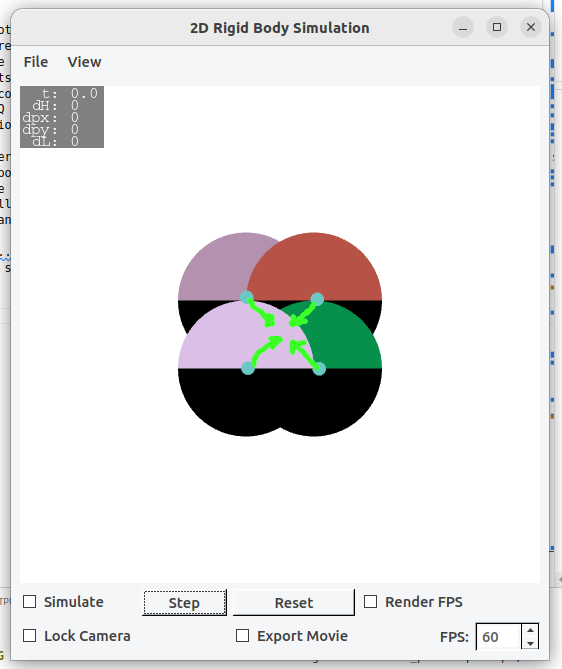
\includegraphics[scale=0.5]{K4_1}

Here I've highlighted the center of the balls and drawn an arrow showing their initial velocities $\dot q^-$.
Even though this isn't a totally realistic/physical scenario, one could instead imagine that all the
something like squares instead with their corners all meeting in the middle. Each object is in 
a simultaneous collision with its 3 other neighbors.


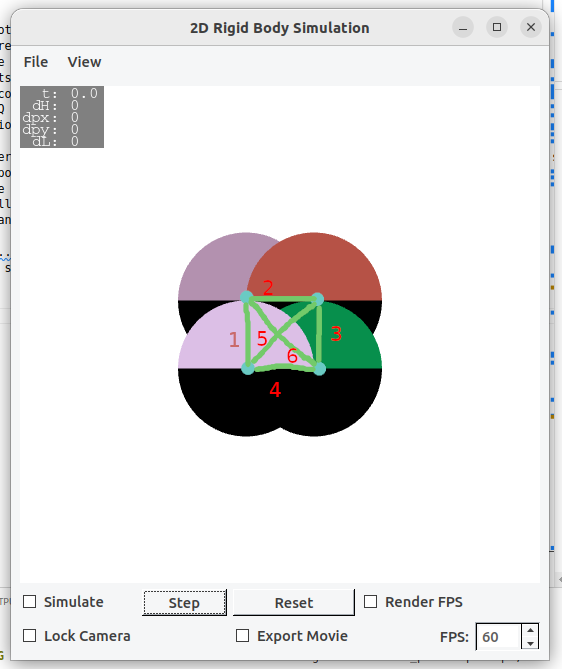
\includegraphics[scale=0.5]{K4_2}

Here I've drawn all the collisions "normals" connecting each pair of colliding balls.
This which shows the K4 graph structure. Each green line drawn corresponds to a column in the
$\GA$ matrix. Each green line also corresponds to an element in $\lambda$.
Each lambda element is an "impulse coefficient" (see the rosi paper)
that can exert force on 2 balls in the direction of
each collision normal (i.e. green line $i$ can be interpreted a like a compressed spring,
whose amount of compression is proportional to the size of the corresponding $\lambda_i$.
The higher $\lambda_i$ is, the higher the force that those 2 balls involved in collision i will
exert on each other).

There are infinite solutions ($\lambda$) to the above picture that result in the same correct exit velocity
of the balls. Either
(a) the 4 $\lambda_i$s corresponding to the 4 outside collisions are $> 0$ with the 2 $\lambda_i$s
corresponding to the inside collisions are $= 0$ (in this case $\pi = \{1, 2, 3, 4\}$),
(b) vice-versa ($\pi = \{5, 6\}$)), or 
(c) any linear combination of the 2 $\pi = \{1, 2, 3, 4, 5, 6\}$.

\section{References}

\begin{itemize}
   \item BOKANOWSKI, OLIVIER, et al. “SOME CONVERGENCE RESULTS FOR HOWARD'S ALGORITHM.” SIAM Journal on Numerical Analysis, vol. 47, no. 4, 2009, pp. 3001–26. JSTOR, \href{http://www.jstor.org/stable/27862763}{http://www.jstor.org/stable/27862763}. Accessed 2023.
   \item Zhang, W. 2022 A Comparison of Linear Solver Methods in Object-Collision Simulations. (See this folder for access)
   \item Wan, K. 2022. URA Report for Computer Simulation of Many Object Collisions. (See this folder for access)
\end{itemize}




\end{document}